% Options for packages loaded elsewhere
\PassOptionsToPackage{unicode}{hyperref}
\PassOptionsToPackage{hyphens}{url}
%
\documentclass[
]{article}
\usepackage{amsmath,amssymb}
\usepackage{iftex}
\ifPDFTeX
  \usepackage[T1]{fontenc}
  \usepackage[utf8]{inputenc}
  \usepackage{textcomp} % provide euro and other symbols
\else % if luatex or xetex
  \usepackage{unicode-math} % this also loads fontspec
  \defaultfontfeatures{Scale=MatchLowercase}
  \defaultfontfeatures[\rmfamily]{Ligatures=TeX,Scale=1}
\fi
\usepackage{lmodern}
\ifPDFTeX\else
  % xetex/luatex font selection
\fi
% Use upquote if available, for straight quotes in verbatim environments
\IfFileExists{upquote.sty}{\usepackage{upquote}}{}
\IfFileExists{microtype.sty}{% use microtype if available
  \usepackage[]{microtype}
  \UseMicrotypeSet[protrusion]{basicmath} % disable protrusion for tt fonts
}{}
\makeatletter
\@ifundefined{KOMAClassName}{% if non-KOMA class
  \IfFileExists{parskip.sty}{%
    \usepackage{parskip}
  }{% else
    \setlength{\parindent}{0pt}
    \setlength{\parskip}{6pt plus 2pt minus 1pt}}
}{% if KOMA class
  \KOMAoptions{parskip=half}}
\makeatother
\usepackage{xcolor}
\usepackage[margin=1in]{geometry}
\usepackage{graphicx}
\makeatletter
\newsavebox\pandoc@box
\newcommand*\pandocbounded[1]{% scales image to fit in text height/width
  \sbox\pandoc@box{#1}%
  \Gscale@div\@tempa{\textheight}{\dimexpr\ht\pandoc@box+\dp\pandoc@box\relax}%
  \Gscale@div\@tempb{\linewidth}{\wd\pandoc@box}%
  \ifdim\@tempb\p@<\@tempa\p@\let\@tempa\@tempb\fi% select the smaller of both
  \ifdim\@tempa\p@<\p@\scalebox{\@tempa}{\usebox\pandoc@box}%
  \else\usebox{\pandoc@box}%
  \fi%
}
% Set default figure placement to htbp
\def\fps@figure{htbp}
\makeatother
\setlength{\emergencystretch}{3em} % prevent overfull lines
\providecommand{\tightlist}{%
  \setlength{\itemsep}{0pt}\setlength{\parskip}{0pt}}
\setcounter{secnumdepth}{-\maxdimen} % remove section numbering
\usepackage{bookmark}
\IfFileExists{xurl.sty}{\usepackage{xurl}}{} % add URL line breaks if available
\urlstyle{same}
\hypersetup{
  pdftitle={Strategic Identification of New Genetic Diversity to Expand Lentil (Lens culinaris Medik.) Production (Using Nepal as an Example)},
  pdfauthor={Derek Michael Wright derek.wright@usask.ca},
  hidelinks,
  pdfcreator={LaTeX via pandoc}}

\title{Strategic Identification of New Genetic Diversity to Expand
Lentil (\emph{Lens culinaris} Medik.) Production (Using Nepal as an
Example)}
\usepackage{etoolbox}
\makeatletter
\providecommand{\subtitle}[1]{% add subtitle to \maketitle
  \apptocmd{\@title}{\par {\large #1 \par}}{}{}
}
\makeatother
\subtitle{\emph{Agronomy}. (2021) 11(10): 1933.
doi.org/10.3390/agronomy11101933}
\author{Derek Michael Wright
\href{mailto:derek.wright@usask.ca}{\nolinkurl{derek.wright@usask.ca}}}
\date{27-09-2021}

\begin{document}
\maketitle

{
\setcounter{tocdepth}{2}
\tableofcontents
}
\begin{center}\rule{0.5\linewidth}{0.5pt}\end{center}

\pagebreak

\begin{quote}
\begin{itemize}
\tightlist
\item
  \href{https://doi.org/10.3390/agronomy11101933}{Sandesh Neupane,
  Rajeev Dhakal, Derek M. Wright, Deny K. Shrestha, Bishnu Dhakal and
  Kirstin E. Bett. \textbf{Strategic Identification of New Genetic
  Diversity to Expand Lentil (\emph{Lens culinaris} Medik.) Production
  (Using Nepal as an Example)}. \emph{Agronomy}. (\textbf{2021}) 11(10):
  1933. doi.org/10.3390/agronomy11101933}
\end{itemize}
\end{quote}

which is a follow-up to:

\begin{quote}
\begin{itemize}
\tightlist
\item
  \href{https://doi.org/10.1002/ppp3.10158}{Derek M. Wright, Sandesh
  Neupane, Taryn Heidecker, Teketel A. Haile, Crystal Chan, Clarice J.
  Coyne, Rebecca J. McGee, Sripada Udupa, Fatima Henkrar, Eleonora
  Barilli, Diego Rubiales, Tania Gioia, Giuseppina Logozzo, Stefania
  Marzario, Reena Mehra, Ashutosh Sarker, Rajeev Dhakal, Babul Anwar,
  Debashish Sarker, Albert Vandenberg \& Kirstin E. Bett
  \textbf{Understanding photothermal interactions can help expand
  production range and increase genetic diversity of lentil (\emph{Lens
  culinaris} Medik.)}. \emph{Plants, People, Planet}. (\textbf{2021})
  3(2): 171-181. doi.org/10.1002/ppp3.10158}
\item
  \url{https://github.com/derekmichaelwright/AGILE_LDP_Phenology}
\end{itemize}
\end{quote}

\begin{center}\rule{0.5\linewidth}{0.5pt}\end{center}

\begin{quote}
\begin{itemize}
\tightlist
\item
  \url{https://github.com/derekmichaelwright/AGILE_LDP_Nepal}
\item
  \href{https://github.com/derekmichaelwright/AGILE_LDP_Nepal/raw/master/README.pdf}{View
  as pdf}
\item
  \href{https://derekmichaelwright.github.io/AGILE_LDP_Nepal/README.html}{View
  as HTML}
\item
  \href{https://derekmichaelwright.github.io/AGILE_LDP_Nepal/Phenology_Vignette.html}{Source
  Code Vignette (Phenology\_Vignette.html)}
\end{itemize}
\end{quote}

\section{AGILE Project}\label{agile-project}

\pandocbounded{\includegraphics[keepaspectratio]{Additional/img_Agile.png}}

\begin{center}\rule{0.5\linewidth}{0.5pt}\end{center}

\section{Figure 1}\label{figure-1}

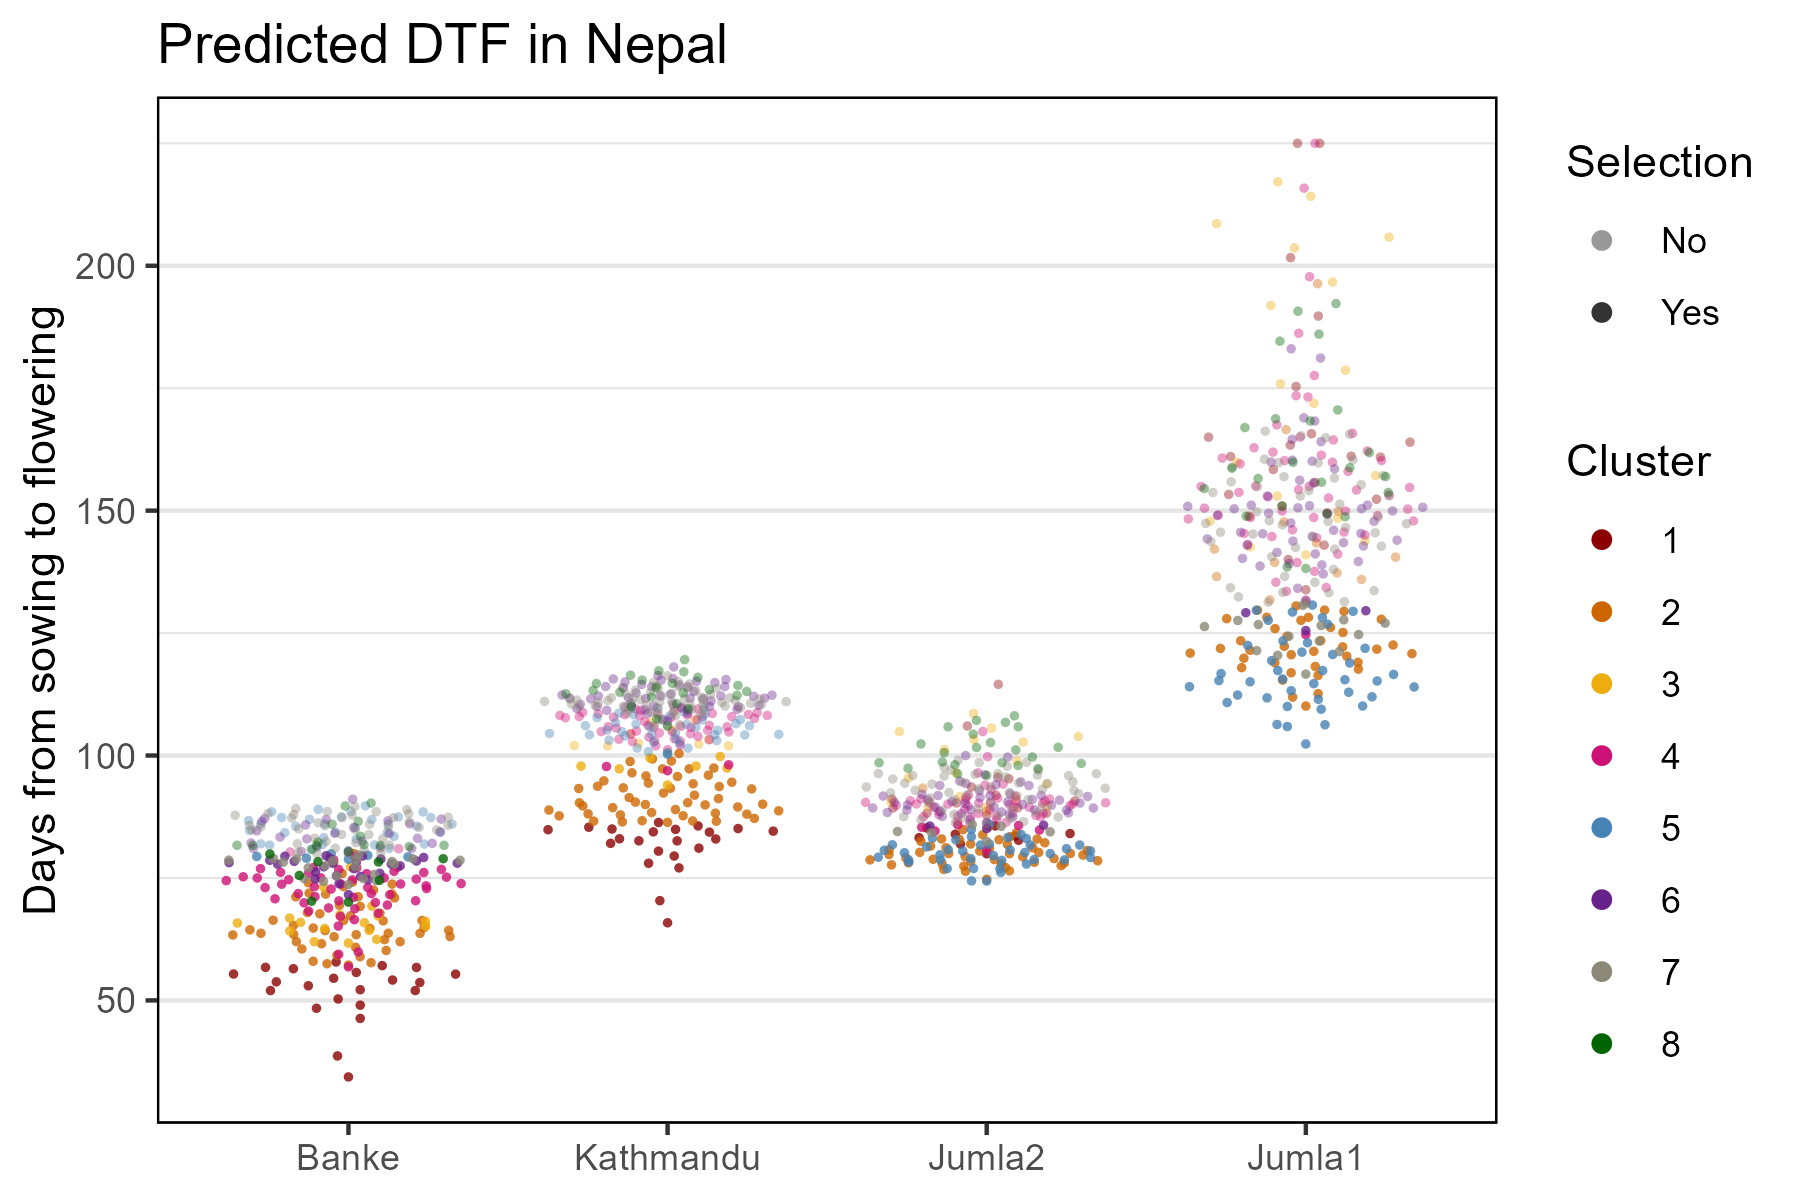
\includegraphics[width=0.9\linewidth,height=\textheight,keepaspectratio]{Figure_01.png}

\begin{center}\rule{0.5\linewidth}{0.5pt}\end{center}

\section{Figure 2}\label{figure-2}

\pandocbounded{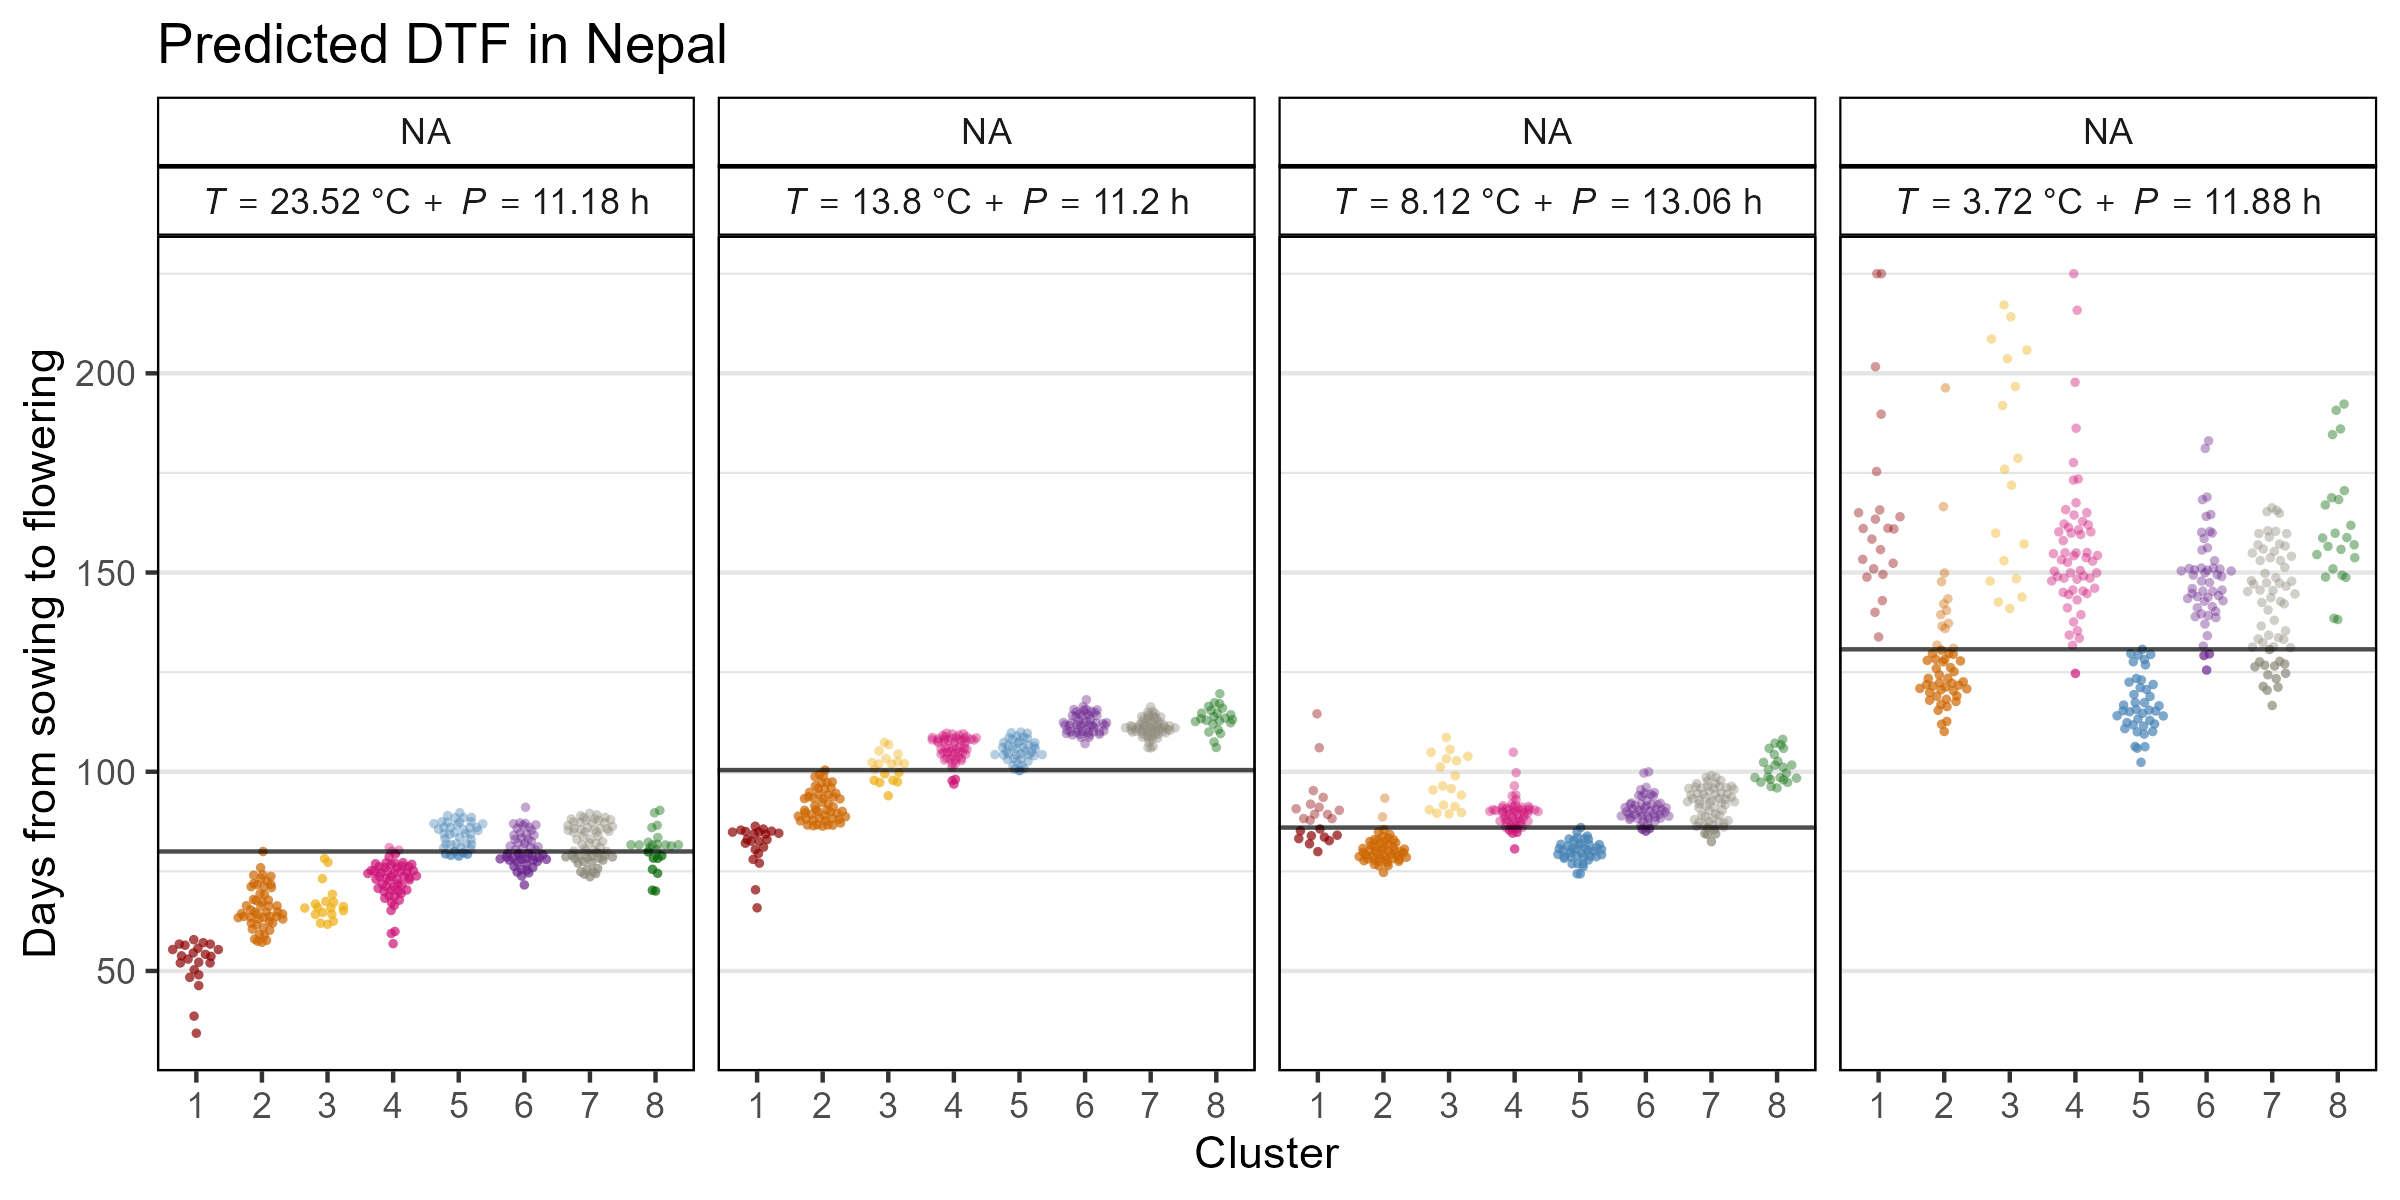
\includegraphics[keepaspectratio]{Figure_02.png}}

\begin{center}\rule{0.5\linewidth}{0.5pt}\end{center}

\section{Figure 3}\label{figure-3}

\pandocbounded{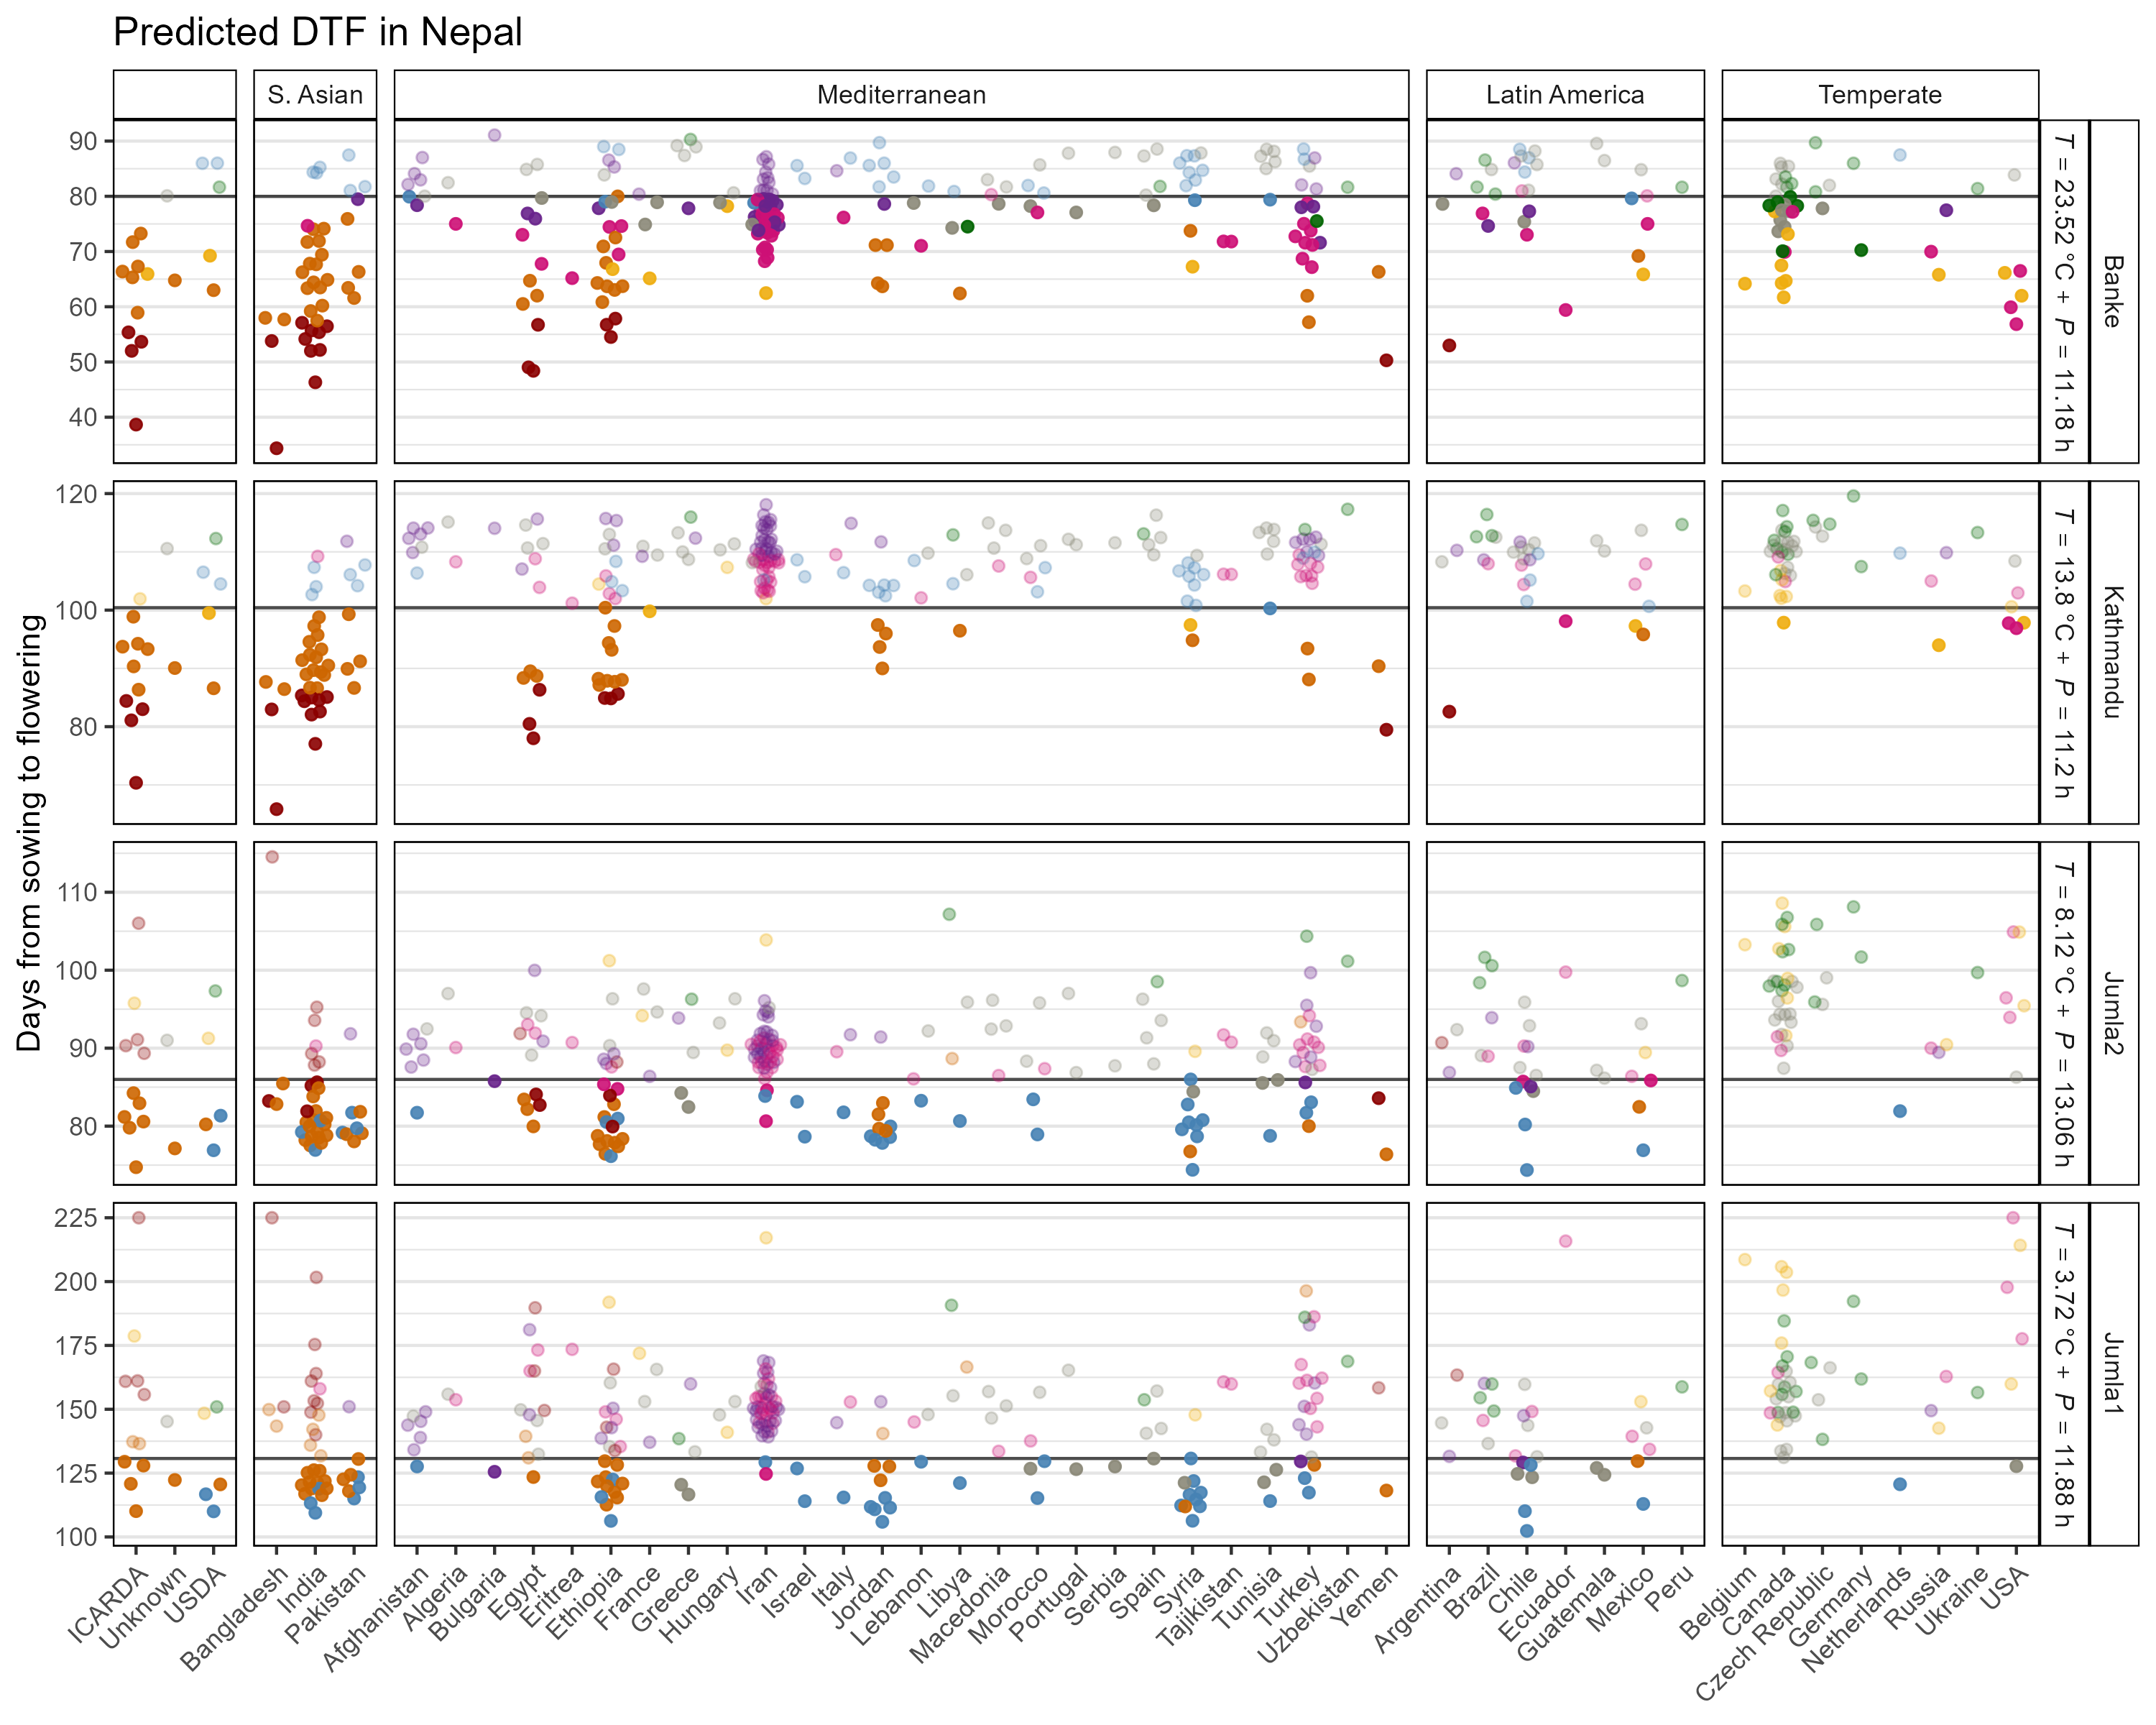
\includegraphics[keepaspectratio]{Figure_03.png}}

\begin{center}\rule{0.5\linewidth}{0.5pt}\end{center}

\pagebreak

\section{Figure 4}\label{figure-4}

\begin{quote}
\begin{itemize}
\tightlist
\item
  \url{https://derekmichaelwright.github.io/AGILE_LDP_Nepal/Figure_04.html}
\end{itemize}
\end{quote}

\pandocbounded{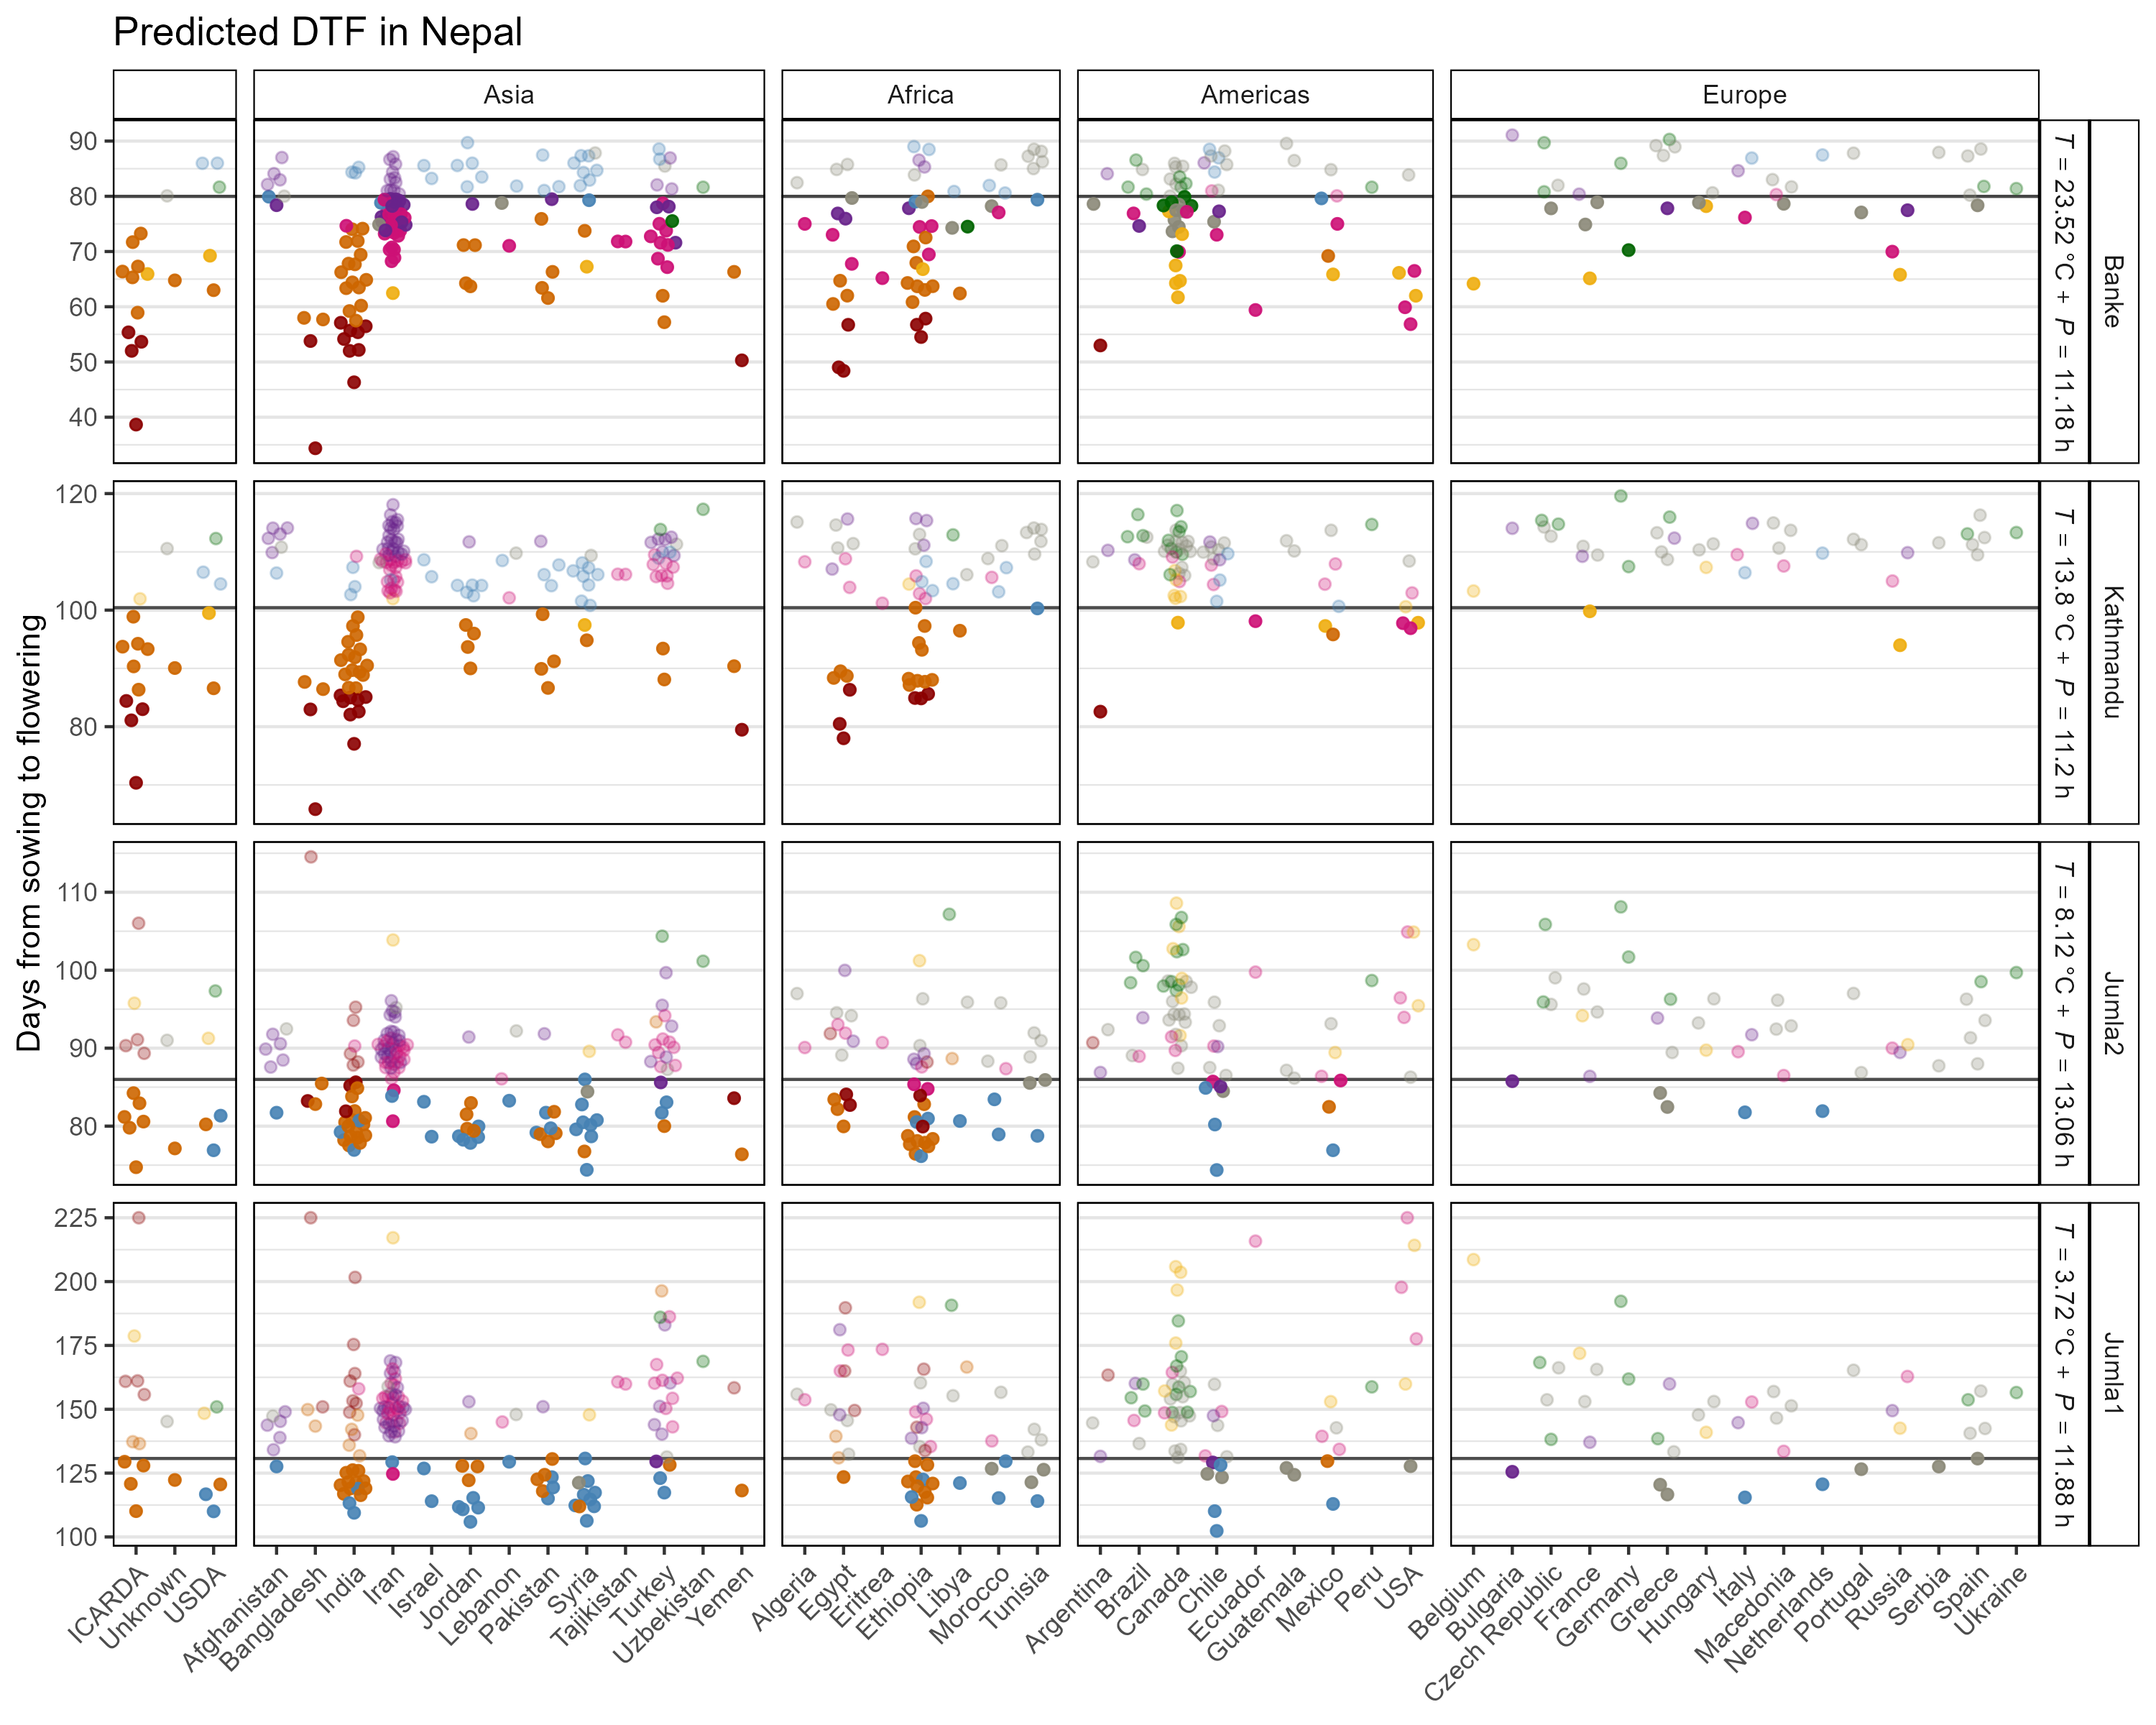
\includegraphics[keepaspectratio]{Figure_04.png}}

\begin{center}\rule{0.5\linewidth}{0.5pt}\end{center}

\section{model\_nepal.csv}\label{model_nepal.csv}

\begin{quote}
\begin{itemize}
\tightlist
\item
  \href{https://raw.githubusercontent.com/derekmichaelwright/AGILE_LDP_Nepal/master/model_nepal.csv}{model\_nepal.csv}
\end{itemize}
\end{quote}

\begin{center}\rule{0.5\linewidth}{0.5pt}\end{center}

© Derek Michael Wright

\end{document}
